\documentclass{report}
\usepackage[utf8]{inputenc}     % for éô
\usepackage[english]{babel}     % for proper word breaking at line ends
\usepackage[a4paper, left=1.5in, right=1.5in, top=1.5in, bottom=1.5in]{geometry}
% for page size and margin settings
\usepackage{graphicx}           % for ?
\usepackage{amsmath,amssymb}    % for better equations
\usepackage{amsthm}             % for better theorem styles
\usepackage{mathtools}          % for greek math symbol formatting
\usepackage{varwidth}
\usepackage{enumitem}           % for control of 'enumerate' numbering
\usepackage{listings}           % for control of 'itemize' spacing
\usepackage{todonotes}          % for clear TODO notes
\usepackage[hidelinks]{hyperref}           % page numbers and '\ref's become clickable
\usepackage{pgfplots}
\usepackage{caption}
\usepackage{parskip}
\usepackage{makecell}
\usepackage{tabularx}

% \pgfplotsset{width=10cm,compat=1.9}


% Listing style

%% Package for colors.
\usepackage{xcolor}
%% Useful colors
\definecolor{blue}{RGB}{0,0,255}
\definecolor{codegreen}{rgb}{0,0.6,0}
\definecolor{codegray}{rgb}{0.5,0.5,0.5}
\definecolor{codepurple}{rgb}{0.58,0,0.82}
\definecolor{backcolour}{rgb}{1,0.973,0.906}
\definecolor{mygray}{gray}{0.96}

%% Code listing style named "mystyle"
\lstdefinestyle{mystyle}{
    backgroundcolor=\color{mygray},
%commentstyle=\color{codegreen},
%keywordstyle=\color{magenta},
%numberstyle=\tiny\color{codegray},
    stringstyle=\color{codepurple},
    basicstyle=\footnotesize,
    breakatwhitespace=false,
    breaklines=true,
    captionpos=b,
    keepspaces=true,
%   numbers=left,                    
    numbersep=5pt,
    showspaces=false,
    showstringspaces=false,
    showtabs=false,
    tabsize=2
}
% "mystyle" code listing set
\lstset{style=mystyle}


%%%%%%%%%%%%%%%%%%%%%%%%%%%%%%%%
%% SET TITLE PAGE VALUES HERE %%
%%%%%%%%%%%%%%%%%%%%%%%%%%%%%%%%
%             ||               %
%             ||               %
%             \/               %

\newcommand{\thesistitle}{Adding authenticated video calling to Pubhubs}
\newcommand{\thesissubtitle}{A design and the need for authenticated video calling}
\newcommand\thesisauthorfirst{Julian van der Horst \\ s1015357}
\newcommand\thesisauthorsecond{}
\newcommand\thesissupervisorfirst{Bart Jacobs}
\newcommand\thesissupervisorsecond{Omar Javed}
\newcommand\thesissecondreaderfirst{TBA}
\newcommand\thesissecondreadersecond{}
\newcommand\thesisdate{May 2023}


%% FOR PDF METADATA
\title{\thesistitle}
\author{\thesisauthorfirst\space\thesisauthorsecond}
\date{\thesisdate}

%%%%%%%%%%%%%%%%%%%%%%%

\begin{document}
\begin{titlepage}
\thispagestyle{empty}
\newcommand{\HRule}{\rule{\linewidth}{0.5mm}}
\center
\textsc{\Large Radboud University Nijmegen}\\[.7cm]

\includegraphics[width=25mm]{img/in_dei_nomine_feliciter}\\[.5cm]
\textsc{Faculty of Science}\\[0.5cm]

\HRule \\[0.4cm]
{ \huge \bfseries \thesistitle}\\[0.1cm]
\textsc{\thesissubtitle}\\
\HRule \\[.5cm]
\textsc{\large Thesis M.Sc. Computing Science}\\[.5cm]

\begin{minipage}{0.4\textwidth}
    \begin{flushleft}
        \large
        \emph{Author:}\\
        \thesisauthorfirst\space \textsc{\thesisauthorsecond}
    \end{flushleft}
\end{minipage}
~
\begin{minipage}{0.4\textwidth}
    \begin{flushright}
        \large
        \emph{Supervisor:} \\
        \thesissupervisorfirst  \\[1em]
        \emph{Daily supervisor:} \\
        \thesissupervisorsecond \\[1em]
        \emph{Second reader:} \\
        \thesissecondreaderfirst\\
        % \thesissecondreadersecond
    \end{flushright}
\end{minipage}\\[4cm]
\vfill
%{\large \thesisdate}\\
{\large \today}\\
\clearpage
\end{titlepage}

\tableofcontents

\newpage
\section*{Abstract}


\chapter{Introduction}


\section{Video conferencing in PubHubs}
Pubhubs is a platform which is currently still looking for a suitable use case. Altough there are many privacy
enhacing features present in Pubhubs, many clients will not use it since it laking features which are required for
their use case. We believe that having the ability to video call within PubHubs can be a very useful feature.
This way the privacy friendly Pubhubs can be used for a lot of applications, like online consultations, online
classes, or just to have a chat with friends. However, currently there are no organisations which are using PubHubs for this. So it is hard to say what the exact requirements are
for video calling in PubHubs. We will make some requirements in terms of privacy, security and usability which we
will be in line with the current PubHubs principles. We will then design a video conferencing solution and implement
this design into a prototype. This prototype will be evaluated on the requirements we have set.


\chapter{Background}
To understand the requirements and design we will first need to understand the current state of PubHubs and the
different frameworks and technologies that we build our design on top of. We will also discuss what precisely we mean
with video conferencing and what the different options are for video conferencing.

\section{PubHubs}
PubHubs, short for Public Hubs, is an alternative community platform that puts public values first
\cite{jacobs_pubhubs_2023}
. Unlike mainstream social media platforms like Instagram or Twitter that focus on individual broadcasting, PubHubs
emulates real-world social dynamics by centering interactions within smaller, community-based hubs. The reasoning
behind that is that this behavior closely resembles normal human interaction, where humans have small groups of
friends and collaborators with whom they interact. The way people experience social media now is very unnatural,
where if they engage with a platform, their posts are shouted into the whole world and are for everyone to see.

“PubHubs is organized as a network of independent hubs, with a shared single-sign-on. Conversations take place in
local hubs (and not globally) and the associated (conversation) data is managed decentrally, within each hub”~
\cite{jacobs_pubhubs_2023}
. Privacy is one of the core values of PubHubs, which can be seen in how it handles identity management. The main
idea of Pubhubs is to allow pseudonymity while maintaining both accountability and the ability to verify certain
attributes of the user.

Pubhubs consists of a central server(Pubhubs central or \textit{PHC}), the Transcriptor (\textit{TS}) and multiple hubs.
When a user registers, they register at Pubhubs central using Yivi (formerly IRMA)\cite{alpar_irma_nodate} by disclosing
certain attributes. When the attributes are verified the user is assigned a global identity by \textit{PHC}.
This global identity is an (Elgamal) encryption of the user identity, which no single entity within Pubhubs
can decrypt, but if the \textit{PHC} and the \textit{TS} work together they can.
In each hub the user will have a local identity, which is derived from the pseudonym.
This local identity is created by multiplying the pseudonym with a hub specific
'psuedonymization' factor which is only known by the
\textit{TS}. This is setup This is done in such a way that \textit{PHC} does not learn to which hub the user is going, while
\textit{TS} does not learn who is visiting the hub.
This way the user can be anonymous within the hub, and even across hubs but whenever the
\textit{PHC} and the \textit{TS} work together they can identify the user for instance when the user is misbehaving.

Pubhubs uses a privacy first design where attributes can be disclosed if the user so chooses.
Hubs can have certain features only be accessed
when certain attributes are disclosed. For example, a hub can require that a user has a certain age before they can
enter a room. The hub can request these attribute using Yivi. The hub can then crypto graphically verify that the
user has the attribute without knowing the actual
value of
the attribute. This way the user can prove that they have the attribute without disclosing the actual value of the
attribute.

In PubHubs all communication is done via Matrix. “Matrix is an open-source network for secure, decentralized
communication” \cite{noauthor_matrixorg_nodate}, which I will expand upon in the next section. PubHubs can be seen as a
layer on top of Matrix, which handles the identity management and adds some extra features like the ability to have
secured rooms.

In Pubhubs the hubs are run by different organizations which typically have a public function, such as
local governments or schools.
These hubs can have different rules or have different features.
To allow this, Pubhubs has a strong divide between Pubhubs central and the different hubs.
This division is even made in the client, where there is a distinction of the global client and the hub client.
The global client enables a user to go from hub to hub and log in, it is
the interface that you see when you visit the Pubhubs website.
Once you enter a hub, the global client loads the hub client in an Iframe. The hub client
is the client that the hub itself deploys. Here, the hubs have full control
over the client and can add plugins or create rooms.
Even in the code base there is a clear distinction between the global client and the hub client.
Although there is a way to communicate between the global client and the hub client, this
is only used to let the hub client know certain settings which are set in the global client.
For example whether the user prefers a light or dark theme.


\section{Video conferencing}
Video conferencing systems have been around since the 60s and 70s when NASA used it to communicate with astronauts
on space flights. It has made its appearance in many science fiction works, where it seemed like a far-off future.
However, in the last decade, video conferencing has become a standard tool for many businesses and individuals.
Popularity increased dramatically during the COVID-19 pandemic, there was a big need for remote work. Immediately,
services like Zoom \cite{Zoom} and Microsoft Teams  \cite{MSTeams} gained widespread adoption. These tools allowed
video conferencing between different remote locations in real-time. However, these tools are not always
privacy-friendly and are mostly setup for convenience and ease of use.

These video call services might include end-to-end encryption but often lack authenticated video conferencing. On
online platforms you can pretend to be anyone you want, it is even rather simple to digitally modify your voice or
face. This has been done in the past by north korean hackers to infiltrate a US organization. Perhaps the need for
authenticated video conferencing is not very apparent, and when calling friends it might not be needed. In contrast, when having an online consultation with your doctor, you
want to be sure that you are actually calling a doctor. This is where authenticated video conferencing comes in.
Authenticated video conferencing is a video call where you can verify that the person you are calling is who they say they are.

If we look at video conferencing from a conceptual perspective, we see that there are multiple conferencing setups.
For this research, we will distinguish three types. Person-to-person (one-on-one), Person-to-person (multiple people
), and speaker-to-audience. We distinguish these types because they all have certain properties that best match with
different technologies. Where in one-on-one we only need to send and receive to one other person, when we are in a
group we need to send and receive data to each member in a call. On the contrary, with speaker-to-audience, we do
not have connections between the individual audience members. The first and second setup are more in line with what
we expect the users of Pubhubs to use video conferencing for, so we will focus on them in this research.

\begin{figure}[!hbt]
\centering
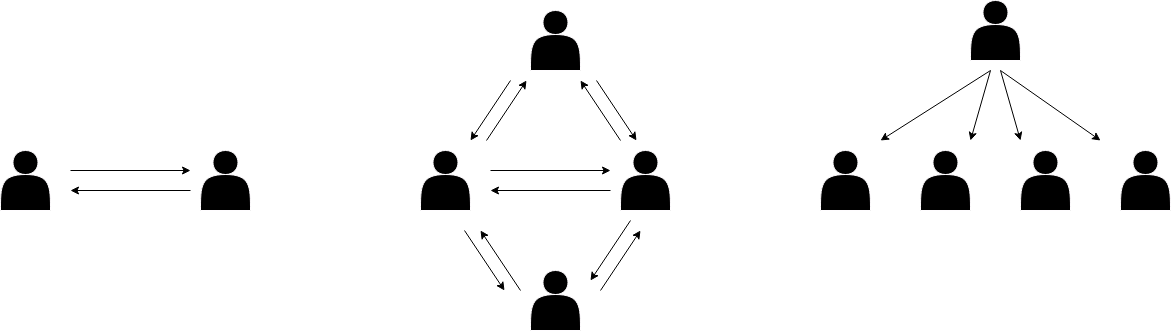
\includegraphics[width=0.7\textwidth]{img/three-types}
\caption{The three types of video conferencing.}
\label{fig:three-types-video-conferencing}
\end{figure}

With video conferencing, people need to send and receive video streams, and we want to do this ideally in real time.
A standard for that is WebRTC, and it is now widely supported in browsers (97.77\% of browser versions used) \cite{
CIUIWEBRTC}. WebRTC is both a protocol and an API that can be used for many things, including video and audio communication.
Matrix even has support for WebRTC and uses it in their main client Element \cite{ELEMENT}. In our
implementation, we will use WebRTC to send video and audio streams. However, to which endpoints do we need
to send these WebRTC streams?

The first option is to send the data in a Peer-to-peer (P2P) network. This means that the people in the call send
their stream to every other person in the call. This ensures that the server has no extra load since it does not
handle any video streams, it simply facilitates the call setup. However, with every extra participant, every user
needs to send/receive more and more data. With every new user we need to use additional computational resources and at
some point, a bottleneck is reached, and loss of data will occur. This is a very privacy-friendly method since the
server has no access to the video conferencing data being sent and the users have full autonomy to choose who can
receive their video data. However, due to the limited number of participants, this solution is not feasible.

Another option would be to have a Multipoint Control Unit (MCU). An MCU takes in many media streams, possibly
converts it to another format and combines these streams into one media stream. This makes it so that it can work
very well with legacy systems, since an MCU can receive various types of media and then output a standardized
output. For example, this would allow a participant to call in from a phone connection while the other participant
is using a desktop application. The MCU has to encode and decode all the incoming media signals, which makes it
costly at large scale, since this is a computationally intensive task. From a security and privacy perspective, this
solution is not ideal, since the server has access to all the unencrypted video and audio data which would mean that
the server could potentially listen in on the call.

Lastly, we have the Selective Forwarding Unit (SFU). An SFU behaves in a way like a switch where it would
selectively forward streams between clients, it does not interact with the video streams so it would work similarly
with encrypted and unencrypted data. From a user perspective, we only need to talk to one server, and we send and
receive all our data through that server. The server simply forwards and thus does not distinguish data coming from
a user or another SFU, which in turn means that we can have multiple SFUs working together to relieve the load. This
can increase the scalability of the system in terms of the number of participants or the quality of the streams when
participants are geographically far apart. An SFU provides a compelling balance of scalability and privacy.


\section{Matrix and Element call}
As mentioned previously, Pubhubs is built upon Matrix. Matrix is an open-source network for secure, decentralized
communication. It is built on an open standard, which means that anyone can build a client or server that is fully
compatible with the Matrix protocol. User can even make proposals to change the protocol, which can then be voted on
by the community. This protocol is continuously changing depending on the use cases of their users. These changes
are then implemented in the multiple implementations of the protocol. The most well-known implementation is Synapse,
which is the reference implementation of the matrix protocol and is also used by Pubhubs.

Pubhubs can be seen as a layer on top of matrix, which handles the identity management and adds some extra features.
A hub will have to deploy a matrix server, in this case synapse, and their hub client. This also means that you can
access hubs using any matrix client, with the downside that some features are not available in all clients, such as
requesting attributes using Yivi. Matrix is the fundamental layer of Pubhubs, and it is important to keep in mind
when designing and implementing new features. When designing the video conferencing solution, we will have to keep
in mind the matrix protocol and only deviate from it when absolutely necessary.

It is important to note that when talking about matrix it sometimes refers to the protocol and sometimes to the
reference implementation. In this research, we will mostly talk about the protocol and not the implementation. These
should be the same but from time to time there are differences for instance when a new feature is in the protocol
but not yet implemented in the reference implementation. We are mostly interested in proposal 3401 \cite{
MATRIX_VIDEO_CALL_PROP}, since here matrix added functionality for video conferencing. This proposal
can be applied to all the above-mentioned server setups and describes a protocol for video conferencing.

The same team that built matrix is also building Element \cite{ELEMENT}, which is an open-source matrix client.
A new feature was added to Element called Element call, which serves as an example implementation of the proposal
mentioned above. They started by using peer-to-peer video conferencing, since this more closely resembled the
decentralized infrastructure of Matrix. However, this turned out to not be the best solution since it allowed for a
maximum of 7 participants and video conferencing required numerous computer  resources from participants. Recently,
they have released a new version that makes use of an open-source SFU called Livekit \cite{LIVEKIT}.

We will use this implementation as a guide during our research; however, we will evaluate all the different choices
made for Element call and deviate from them based on the requirements of PubHubs. When using Livekit we can easily
implement features like noise suppression or video simulcast (Sending multiple video streams with different
qualities, to dynamically choose the quality according to a user's internet connection). On the other hand it
also makes pubhubs dependent on Livekit, which is a third party service.


\chapter{Requirements}
\section{CIA}
The CIA triad is a model designed to guide policies for information security within an organization. The model
consists of three core principles: Confidentiality, Integrity, and Availability. These principles are used to
evaluate the security of an information system. We will use this model to evaluate the requirements for the video
conferencing solution.

\subsection{Confidentiality}
Confidentiality is the principle that information is not made available or disclosed to unauthorized individuals,
entities, or processes. In the context of video conferencing, this means that the video and audio data should only
be available to the participants in the call. This means that the server should not have access to the video and
that only the participants in the call should be able to decrypt the video and audio data. Meaning we need end-to-end
encryption.

We will also want to have forward secrecy, meaning that new participants cannot decrypt previous messages. This
means that when a new participant joins the call, they should not be able to decrypt the video and audio data from
before they joined the call. We do not want to have information shared in the call to be decrypted by participant who
joined later.

\subsection{Integrity}
Integrity is the principle that information is protected from unauthorized modification. In the context of video
conferencing, this means that the video and audio data should not be modified by unauthorized individuals, entities,
or processes. We can achieve this by having an authenticated encryption scheme, such that we can verify that the
data is coming from the right participant and has not been tampered with.

\subsection{Availability}
Availability is the principle that information is available and accessible when needed by authorized individuals,
entities, or processes. In the context of Pubhubs, this means that the video conferencing solution should be able to
handle a large number of participants without compromising the functionality of the rest of Pubhubs. This means that
the video conferencing solution should not overload the server and should be able to scale horizontally to handle
more participants.


\section{Code isolation}
Pubhubs is a platform that is still in development and is constantly changing. This means that the video
conferencing solution should be able to adapt to these changes. Pubhubs is also meant as a very configurable platform
where hubs can enable or disable certain features. This means that the video conferencing solution should be able to
be disabled without affecting the rest of Pubhubs.


\todo{Andere manieren van user profile building}
\todo{Device spoofing maybe}


\chapter{Proposed solution}
\begin{figure}[!hbt]
\centering
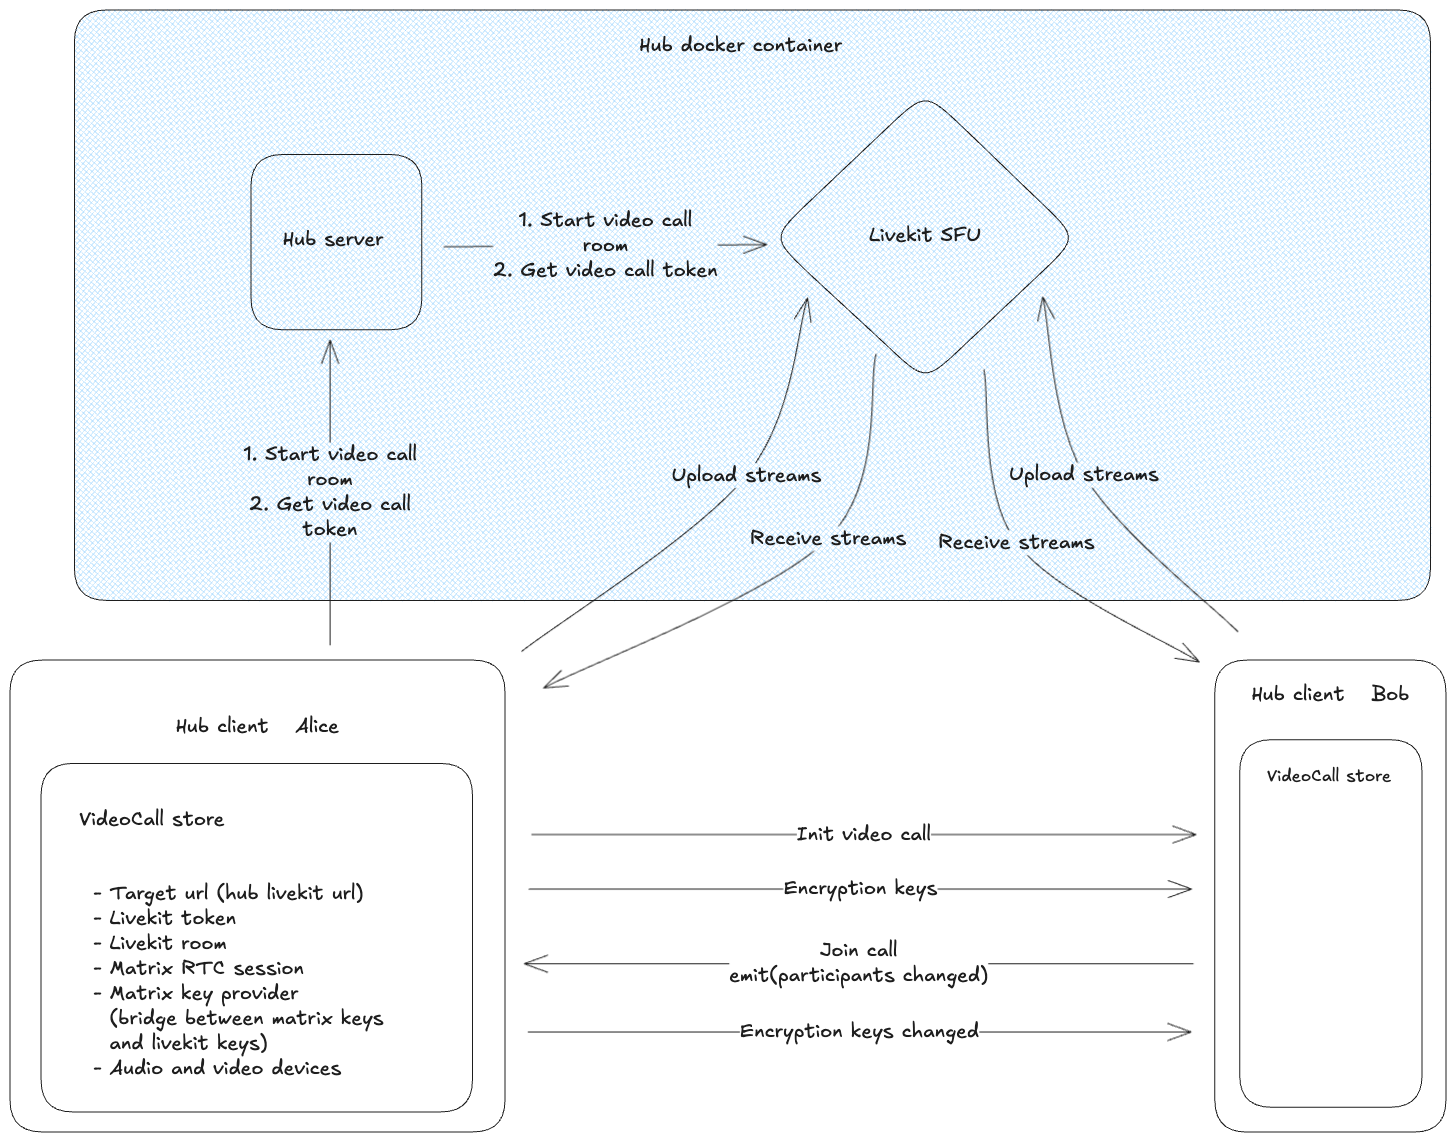
\includegraphics[width=0.8\textwidth]{img/PH_videocall.excalidraw.png}
\caption{Caption}
\label{fig:video-conference-setup}
\end{figure}

This setup can be fully removed from a hub, should a hub not want video conferencing. It is standing on its own and
can be toggled on or off using a feature flag. Everything is programmed in such a way that it is completely isolated
from the rest of Pubhubs.


\section{Server setup}
We first consider the Hub server, which will now also need to deploy a Livekit server instance. This livekit server
functions as an SFU and will forward all the video and audio traffic between the different clients. This server will
not see the video data which is sent since they are encrypted and the server does not have access to the keys. The
only thing that the livekit server sees it the local pseudonym of the user, which the hub server already knows and
thus does not leak additional data. The livekit server can handle a lot of traffic but when the hub is very large
and has a lot of video calls, it might be a good idea to have a separate livekit server. This way the hub server
will not be overloaded with video traffic and can still serve the rest of the users. The livekit server can also
scale horizontally to handle more traffic. This requires no extra programming but it is simply a matter of deploying
more livekit servers and configuring them to work together. Livekit provides a CLI tool which can give an
indication what the maximum amount of users is that a livekit server can handle. This way the hub server can decide
when to scale up the livekit server.

To give some indication, a livekit server running in a google cloud compute instance with 16 cores (
c2-standard-16), has around 85 \% CPU utilization when 150 users with 720p video and audio are connected
\cite{noauthor_benchmarking_nodate}. The hub sever can also choose to completely outsource the livekit server.
Livekit provides a paid service where they will host the livekit server for you. This service scales
automatically and the servers are distributed globally. This way the users will always have a proper low
latency connection to a livekit server. This however is a tradeoff between privacy and ease of use. When using
the livekit service, livekit will not have access to the video conferencing data, but they will have access to
the hub pseudonyms of the users and other metadata. This is a tradeoff that the hub server will have to make,
but we do not recommend that they do.

We have also set up a new route and web request handler on the hub server.
\texttt{GET /\_synapse/client/videocall} We use this endpoint ot authenticate the user and set up a video call
in livekit. For that we need to create a room and add the user to that room. We can add all sorts of checks to allow
a user to join a room,like checking if the user is in the room, if the room exists, if the user is allowed to
join the room, etc. The requirements are not set in stone and can be changed to fit the needs of the hub server.
For now we check if the user is allowed to join the room and otherwise return a 403.

The hub server authenticates the user by checking the pubhubs authentication token on the request. These tokens are
the same as when a user request any other data from the hub server. The response of this call will be an
access token from livekit for this pseudonym and for this room. This token can then be used by livekit to
authenticate the user. Ideally we would not have another token which would in turn be used to authenticate the
user, however this allows us to have a separation between the hub server and the livekit server. This way we can
even host the livekit server on a different server than the hub server. This is a good idea since the
livekit server will have a lot of high bandwidth traffic and we do not want to overload the hub server with
this traffic, essentially denying service to other user because we have a large video call. The user then
has the livekit token, which it will provide when sending and receiving data from the SFU. Non authenticated
media will be rejected.


\section{Video conferencing flow}
Here we deviate somewhat from the original matrix specification. Since the spec also includes a protocol for
sharing which media devices are being used, we will not use this since livekit can handle this for us. Instead
of sharing a lot of information about our setup and endpoints, we only need to know that a call has started and
if the call is encrypted we need to know the encryption keys of the participants. Livekit will provide us with
an endpoint where we can send and receive our data, which in turn forwards it to the others in our room. We
will thus only use the matrix protocol for setting up the room and sending the keys. This approach is also what
matrix intends to do moving forward, as they have specified in a presentation \TODO{find presentation}. The
matrix team now support both solutions in their client sdk.

\begin{figure}
\centering
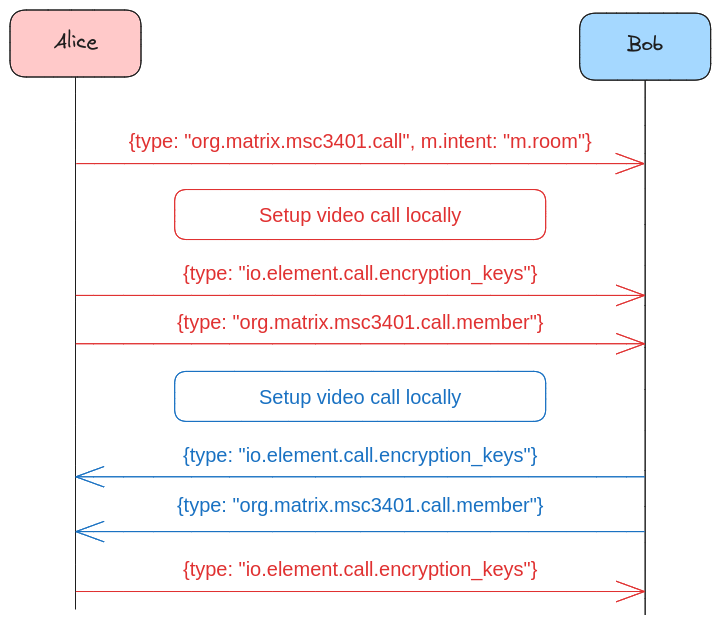
\includegraphics[width=0.6\textwidth]{img/Callflow.excalidraw.png}
\caption{The video conferencing flow}
\label{fig:video-conference-flow}
\end{figure}

When Alice wants to start a call with Bob, she will sent a call event with an intent. This intent can be
everything from having the room automatically join to ringing the other participants. We did not implement
these different behaviours since it was out of scope. After this her client will setup the video conferencing
screen, this is where she can choose her camera and microphone. When she is ready Alice will send her encryption
keys and will send to the others that she is a member of the call. She will then wait for any changes to the
participants
if that happens she will update her keys and send them to the others.

Bob will receive the call event and decides to join the call. His client will setup the video conferencing
screen where he can choose his camera and microphone. When he is ready Bob will send his encryption keys and will
send to the others that he is a member of the call. Since Alice can see that there is a new participant she will
update her keys and send them to Bob. Now they have all the keys of all the participants and they can decrypt their
video and audio streams.

Alice sent her keys twice which is not strictly necessary, however using this we can have a simple code base
without having to check if the keys are already sent. The setup of a call is now the same, regardless whether
the call is new or already ongoing. This makes the code easier to understand and maintain.

Although the keys are sent in the clear, they are only sent to the other participants in the call. This means that
only the participants in the call can decrypt the video and audio streams. Ideally we would send private
messages to the participants in the call, which is also possible within matrix. However this is not the default
currently since matrix is transitioning to a new end-to-end encryption library which is not yet fully implemented.
We have been in contact with the matrix team and they are working on this feature, so we decided to leave the code
as is and wait for the new implementation. This means that until we have the new implementation we do not have
full forward secrecy.


\section{Encryption}

For video calling, we want to have end-to-end encryption. This encryption should ideally also have forward secrecy.
Meaning that new participants cannot decrypt previous messages. Livekit provided an e2ee worker, which locally
encrypts and decrypts incoming messages. This worker is a web worker, which is a separate thread that runs in the
background. This way the main thread is not blocked by the encryption and decryption process. The worker uses the
WebCrypto API, which is a widely used and tested API for encryption and decryption. These APIs are now common in all
modern browsers, so we can be sure that the encryption and decryption will work on all devices.

Livekit uses Advanced Encryption Standard cipher in Galois/Counter Mode (AES-GCM), to encrypt and authenticate the
frames. This is a widely used and researched block cipher which is even used by Netflix \TODO{Add ref, is in Zotero}
).
It is also very fast, which is important for video calling. The key is derived from the key that is sent by the
participants in the call. This key is then used to decrypt the video and audio frames from the other participants.

\TODO{UItbreiden en aan elkaar plakken}

For the encryption to work, we do need the keys from all participants. To get these keys we followed the matrix
specification for ease of implementation and code sustainability. As of the writing, matrix is in the middle of
transitioning to a
new spec where the client can more directly request, revoke and rotate keys of the participants. Although this would
be a better solution, we decided to stick with the current implementation since the new implementation is not yet
fully implemented.

Whenever we are in a call we subscribe to a Matrix\_RTC\_Session. This session handles memberships and
properties of a session. This will give us messages when a new user is added or when the keys are updated.
Whenever we get an updated key message from the rtc\_session, we pass it through livekit, which in turn updates
the keys and derives new keys from that key. It simply takes the key from matrix\_rtc and uses
that as a seed. Although it is not implemented, users can also rotate their keys. This is a feature that is
supported by livekit, but we did not implement it since it was out of scope. Other complex key generation schemes
are also possible and can very easily be implemented.

Currently, the matrix team has enabled e2ee, but they used a now old C++ implementation of Olm. They are now moving
toward their new Rust implementation of it. It is not completely up to par, but the features we need are here. We
don't need much for the encryption of video calls, however, when we use the crypto library to create random keys
which we will send and use to encrypt our sources. Since we need to initialize the matrix crypto library, we can
very easily enable end-to-end encryption for other messages in Pubhubs. We have done some experiments with this,
which we will discuss in a later chapter.


\section{Front end setup}
As mentioned before, the video conferencing client is completely separate from the rest of Pubhubs. This means that
the video conferencing solution can be easily enabled using a feature flag. This also means that the code is
written in a way such that it is isolated.

The Iframe has the sandbox attribute set, meaning that some browser features cannot be accessed from within the
iframe. This turned out to be a problem, when requesting Camera and Microphone access, since these are considered
secure attributes. We can request these permissions in the global client; however, this does in essence allow the
hub client to identify the users across hubs. The hub can create a profile of users by saving which video
conferencing devices are connected. We could perhaps work out a way to spoof the names of the devices, but this
would impact the user experience by making it difficult to see which device is your preferred one.

\chapter{Evaluation}
\section{Privacy}

% \newpage
% \section{Research question}
% The main research question will be \textbf{“How can we design and implement an authenticated video conferencing
%     solution within PubHubs that balances privacy, security, and usability?”}. This main question creates several
%     sub-questions. We will divide these up into three different categories.

% \textbf{Privacy}
% For Pubhubs privacy is one of their core values and during the creation and development of Pubhubs certain
%     decisions have been made regarding privacy. These decision should be considered and can be formulated into
%     these sub-questions:

% — What information or metadata should we allow leaking to achieve authenticated video conferencing, regarding the
%     current Pubhubs privacy principles?

% — How can we balance essential call features, like visible call status, with a commitment to user privacy?

% \textbf{Encryption}
% One of the foremost considerations in GDPR compliance for video conferencing is the implementation of end-to-end
%     data encryption. This requires an encryption scheme which is user-friendly, has low computational overhead, and
%     still has appropriate security.

% — What encryption scheme is best suited for authenticated video conferencing in Pubhubs, weighing user experience
%     and computational overhead while ensuring optimal security?

% \textbf{Development}
% While doing the research and writing the code for it, we should also keep in mind the current development setup for
%     PubHubs. This means that we should keep in mind which technologies they are using now and remain in those
%     ecosystems. This makes it so that the code can be more easily maintained in the future. Pubhubs allows hubs to
%     create their own version of the hub client, which should be considered when creating the video conferencing
%     client.

% — How can we develop a video conferencing prototype within the existing Pubhubs ecosystem, while simultaneously
%     considering different hub client implementations?


\chapter{Future work}

% speaker-to-audience
% Different authentication methods

\bibliographystyle{plain}
\bibliography{references.bib}

\printbibliography

\end{document}